
\textbf{Локализация}. The fundamental opposite of thermalization is localization. It happens that the system retains information about the initial conditions even with $t \to \infty$ (fig. \ref{fig:BASE}, \blue{blue curve}) and $A = A(\psi_0)$. For example, we can divide the system into two equal subsystems$\Omega_1,\, \Omega_2$, populate only $\Omega_1$ and monitor the contrast
\begin{equation*}
	\mathcal{I} = \frac{N_{\Omega_1}-N_{\Omega_2}}{N_{\Omega_1}+N_{\Omega_2}}.
\end{equation*}
So in \cite{schreiber_observation_2015} in 1D the even lattice nodes (fig. \ref{fig:loc1}) were chosen as $\Omega_1$, and in \cite{Choi_2016} in 2D the left side of the system was taken as $\Omega_1$ ( fig.\ref{fig:loc2D1}). Just for $\mathcal{I}(t)$ the declared thermal behavior is already visible when $\mathcal{I}(t \gg \tth) \approx 0$, but at some point there is a transition to localization and $ \mathcal{I} (t \gg \tth) \approx \const > 0$. This behavior is typical when frozen noise $\Delta > 0$ is added to the system; this effect was first described by Anderson \cite{PhysRev.109.1492} for non-interacting particles (AL - Anderson Localization). In the case of interaction (MBL - Many Body Localization), the theoretical description, as far as I know, remains an open task and therefore is of great interest for experiment.

For a single-particle problem, it would be logical to assume that this behavior arises due to the localization of eigenfunctions. Indeed, in fig. \ref{fig:loc1} the eigenstates of the single-particle 1D Hamiltonian \eqref{9:model} are presented at different noise levels $\Delta$.
% Здесь хотелось бы добавить немного конкретики, в этом эссе будет рассматриваться Hubbard model (которая иногда сводится к Heisenberg model, см. приложение):



\begin{figure}[h]
    \centering
    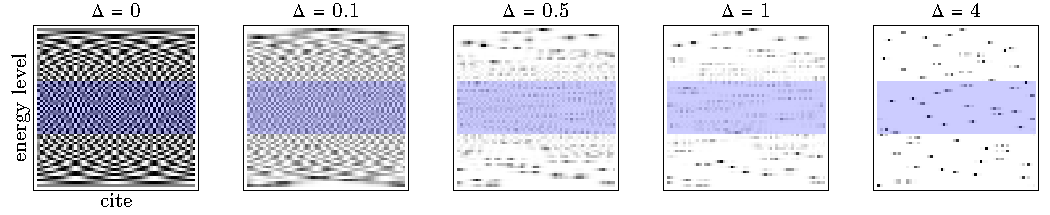
\includegraphics{imgs/evecs.pdf}
    \caption{Eigenvectors for $L=60$ and $N=1$}
    \label{fig:loc1}
\end{figure}

